This test case is fully identical to the one given in \cite{voGaussianMixtureProbability2006} and demonstrates the accuracy of the implementation by showing that the results obtained by the authors of the original paper are reproducible.

In this scenario, two objects are born at the same time at $k=1$ and follow independent linear paths. The initial state vectors of these objects are the following:

\begin{equation}
    \svecat{x}{1}{(1)} = \begin{bmatrix}
        250.0 \\
        250.0 \\
        2.5 \\
        -12.0
    \end{bmatrix},
    \qquad
    \svecat{x}{1}{(2)} = \begin{bmatrix}
        -250.0 \\
        -250.0 \\
        12 \\
        -2.5
    \end{bmatrix}.
\end{equation}

At a certain moment, their tracks cross. Both objects disappear at time $k=100$. Therefore, the number of objects remains constant throughout the simulation, with two objects present at all times. The paths of both objects are shown in Figure \ref{fig:c1-scenario}. The arrows show the direction of movement, and the position of the arrowhead denotes the position of the object death. The circles on the other side of the line illustrate the location of the target birth.

\begin{figure*}
    \centering
    \begin{subfigure}[]{0.48\linewidth}
        \centering
        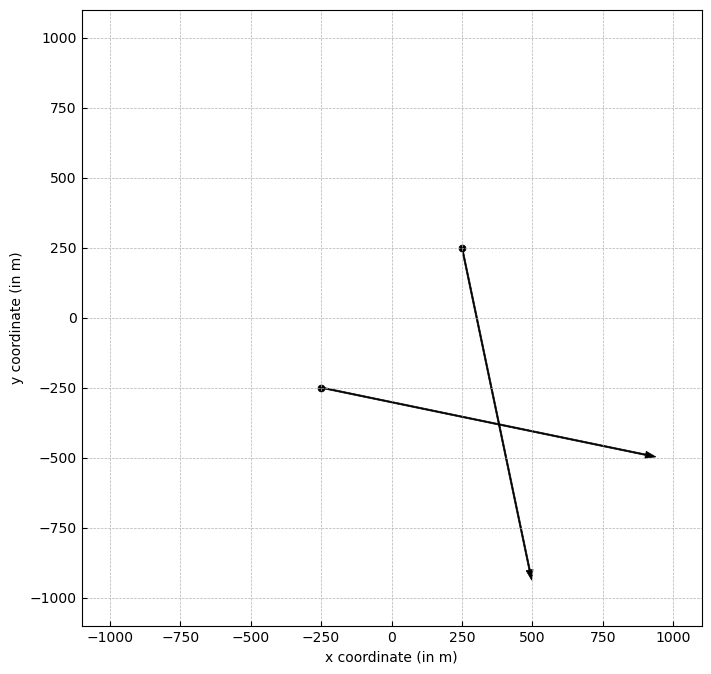
\includegraphics[width=\linewidth]{figures/c1-tracks.png}
    \end{subfigure}
    \hfill
    \begin{subfigure}[]{0.48\linewidth}
        \centering
        \begin{subfigure}[t]{\linewidth}
            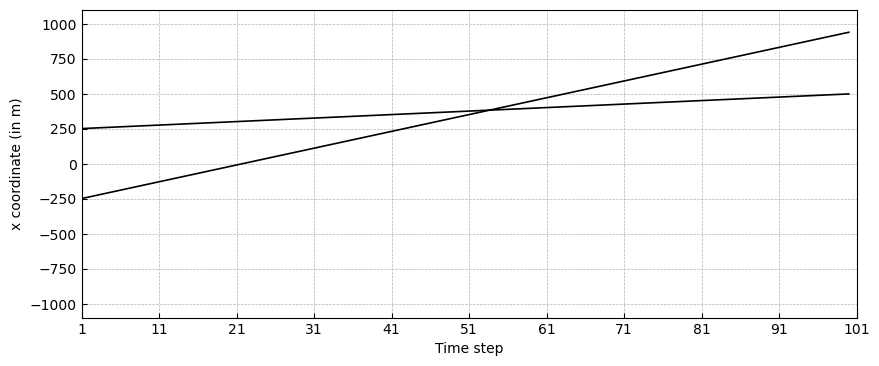
\includegraphics[width=\linewidth]{figures/c1-coord-x.png}
        \end{subfigure}
        \vfill\par
        \begin{subfigure}[b]{\linewidth}
            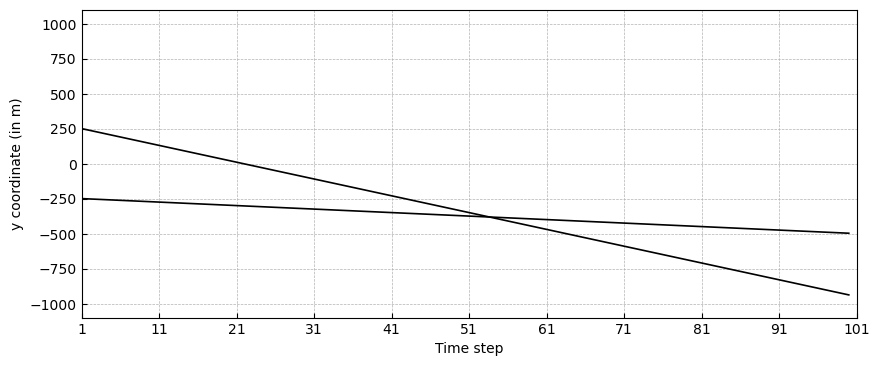
\includegraphics[width=\linewidth]{figures/c1-coord-y.png}
        \end{subfigure}
    \end{subfigure}
  \caption[True tracks of objects in the (C1) scenario.]{The (C1) scenario. In the left figure, we see the tracks of two objects in the 2D space, locations of their births (black circles) and deaths (arrow heads). In the right figure, we see how each coordinate of the tracks of both objects changes over time. We can see that the tracks of two objects intersect at time $k=53$.}
  \label{fig:c1-scenario}
\end{figure*}

Finally, the initial Gaussian mixture of the birth intensity in this scenario is given by:

\begin{equation}
    \gamma_k(\mathbf{x}) = 0.1 \mathscr{N}\left( \mathbf{x}; \svecat{m}{\gamma}{(1)}, \vecat{P}{\gamma} \right)
        + 0.1 \mathscr{N}\left( \mathbf{x}; \svecat{m}{\gamma}{(2)}, \vecat{P}{\gamma} \right),
\end{equation}

\noindent where:

\begin{equation}
    \svecat{m}{\gamma}{(1)} = \begin{bmatrix}
        250 \\
        250 \\
        0 \\
        0 \\
    \end{bmatrix},
    \qquad
    \svecat{m}{\gamma}{(2)} = \begin{bmatrix}
        -250 \\
        -250 \\
        0 \\
        0 \\
    \end{bmatrix},
    \qquad
    \vecat{P}{\gamma} = \begin{bmatrix}
        100 & 0     & 0     & 0     \\
        0   & 100   & 0     & 0     \\
        0   & 0     & 25    & 0     \\
        0   & 0     & 0     & 25    \\
    \end{bmatrix}.
\end{equation}
